% FTC Simulator technical report.
% Build:  latexmk -pdf main.tex      (writes main.pdf here; copy it to docs/static/pdfs/ftc-sim-report.pdf)
% Figures: figures/*.pdf come from docs/figures/*.svg through tools/svg2pdf.mjs (see that file).
% Converted from the report doc's Markdown export on 2026-11-18; this file is now the paper's source.
\documentclass[10pt,twocolumn,letterpaper]{article}
\usepackage{springphy-report}

\reportdate{2026-11-19}
\reportlogo{figures/springphy-wordmark.png}
\reporttitle{Programming the Robot Before It Exists: A Physics Simulator for FIRST Tech Challenge}
\reportshorttitle{Programming the Robot Before It Exists: A Physics Simulator for FIRST Tech Challenge}
\reportauthors{Lening Li\textsuperscript{1} and Na Li\textsuperscript{1}}
\reportaffiliations{\textsuperscript{1}Springphy AI}
\reportnote{Technical report, draft}
\reportfootnote{Code: \url{https://github.com/leelening/ftc-sim}. Project page: \url{https://leelening.github.io/ftc-sim/}.}

\begin{document}
\makereporttitle

\begin{abstract}
FIRST Tech Challenge (FTC) teams build a new robot for a new game every season, and their programmers rarely have a working robot to test on. Existing FTC simulators are mainly teaching tools, and none that we found documents a model of the robot hub’s control loops or of the time each hardware call takes. We present a physics-based simulator for FTC robots playing the 2026–27 game, BIOBUZZ. It models the field and its structures, the 56 game pieces, the two bistable HIVES, and up to four robots with their motors, mechanisms, sensors and webcams. A robot is described in a JSON file or imported from its CAD model, in which case its arms, slides and hoods become bodies on joints. Everything specific to one game is kept in a season pack, and the 2025–26 game, DECODE, is included as a second pack. Matches are run from a browser version of the Driver Station.

Rigid-body physics runs in ODE4j with a 1~ms step, paced to the wall clock; on a desktop computer, four robots and all the game pieces run at 1.7 to 2.0 times real time. We model mecanum wheels with anisotropic contact friction, motors with their datasheet torque–speed curves, and the REV hub's firmware control loops, battery sag and hardware-call timing. The HIVE model is calibrated against the tipping table in FIRST's Event Field Setup Guide and against balls launched by a simulated robot. Webcam frames are rendered in software and passed to FIRST's own AprilTag pipeline; on these frames, which have no lens distortion or noise, the tag positions it reports in our tests are within 2~mm of ground truth.

Teams drive the simulated robots with their own robot code, compiled unmodified, and with real gamepads. We describe the models, a test suite that runs on Windows, Linux and macOS, and a planned comparison with a physical robot and field. The code is open source under the MIT license.
\end{abstract}
\keywords{FIRST Tech Challenge, robot simulation, rigid-body physics, reality gap, AprilTag, robotics education}

\begin{figure}[t]
\centering
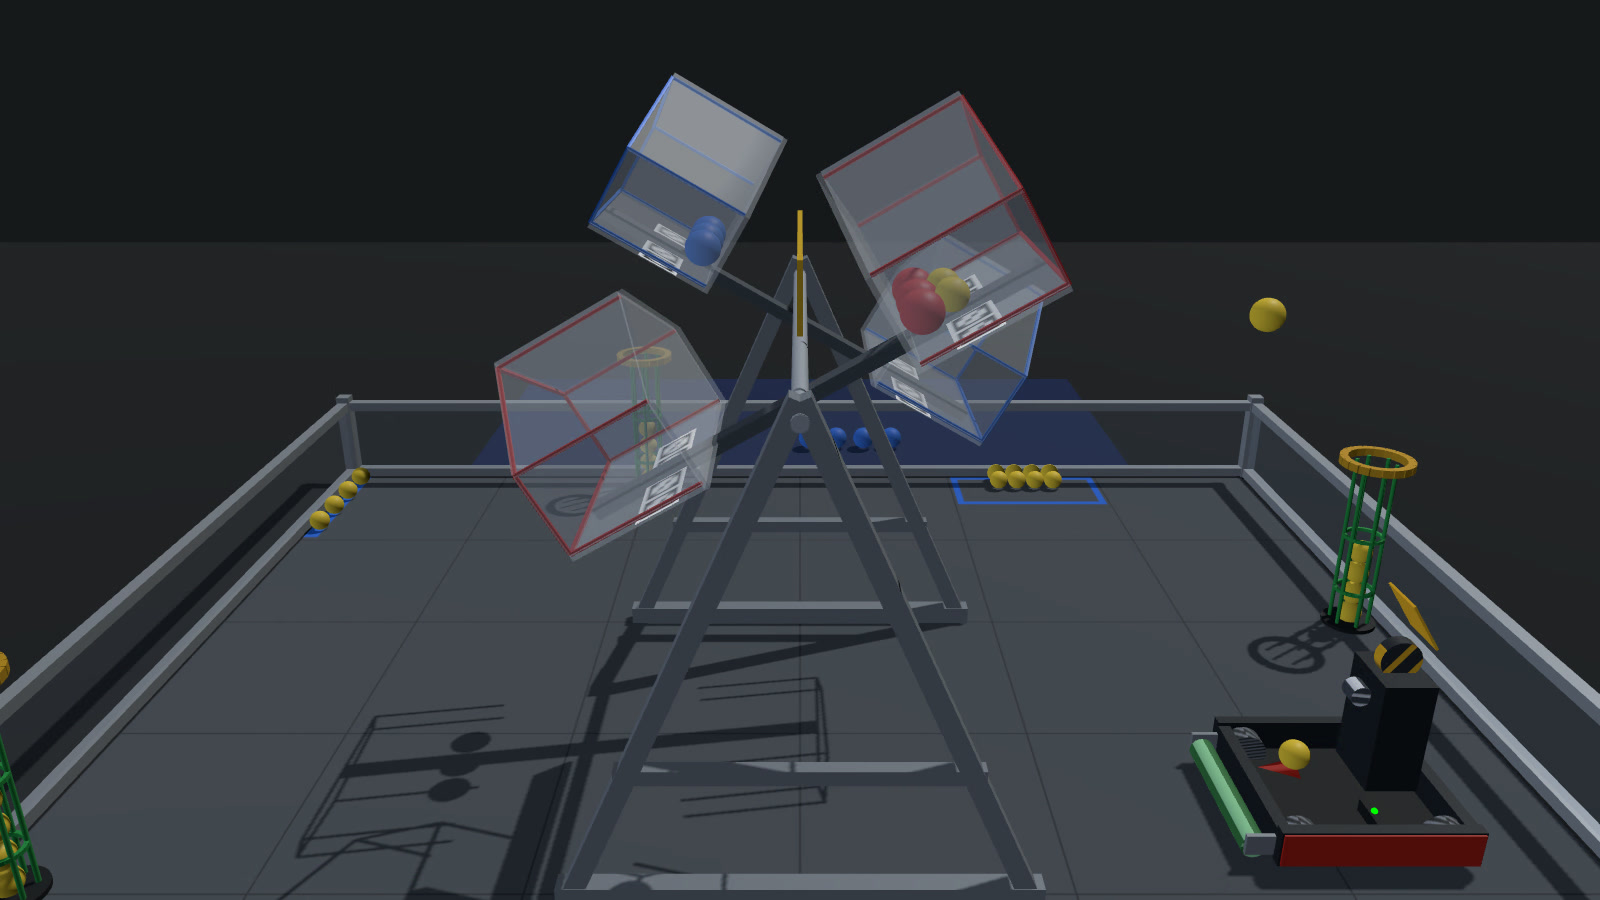
\includegraphics[width=\columnwidth]{figures/teaser.jpg}
\caption{\textbf{A simulated robot running the bundled BIOBUZZ TeleOp.} It spins up its launcher and shoots POLLEN
into the red HIVE's open CELL. With 3 NECTAR already inside, the CELL holds 2 POLLEN; the third tips the HIVE, as
FIRST's field setup guide specifies (\cref{sec:field}).}\label{fig:teaser}
\end{figure}

\section{Introduction}\label{sec:intro}

Every season, FTC teams build and program a new robot for a new game, and programmers rarely get much time with a working robot. For most of the build season the robot is partly assembled, several programmers share it, and the last hours before an event usually go to mechanical repairs. A simulator lets programmers write autonomous routines and tune control loops, and lets drivers practice, before the robot is finished or while it is being rebuilt.

\paragraph{FTC in brief.} An FTC robot is controlled by a REV Control Hub, often with an Expansion Hub, which drives the motors and servos and reads the sensors. Teams program it in Java against FIRST’s SDK \citep{first2026ftcrobotcontroller}. Each program is an OpMode, kept in the TeamCode module of an FtcRobotController project and usually built with Android Studio. A driver picks and starts OpModes on the Driver Station app and drives with gamepads. Two alliances of two robots play each match, which opens with a 30-second autonomous period.

Simulation is widely used in robotics \citep{choi2021simulation}, but behavior that works in simulation can fail on hardware when the model is wrong, a problem known as the reality gap \citep{jakobi1995noise,koos2013transferability}. Robotics developers use simulation for testing but name fidelity and setup cost as its main problems \citep{afzal2021simulation}, although many robot bugs can be reproduced in simulation \citep{timperley2018crashing}. We expect that, for FTC, whether a routine works on the robot depends mostly on the drivetrain, the motors, the hub's control loops, sensor behavior and timing, and the game elements. These are the parts we model in most detail; experiment E5 (\cref{sec:evaluation}) tests which of them matter.

Existing FTC simulators are mainly teaching tools (\cref{sec:related}). None that we found documents a model of the hub's firmware control loops or of hardware-call timing, and none models the 2026–27 game. Our simulator is built for the BIOBUZZ season. Because the game changes every year, the field and the game are kept out of the engine, in a season pack that can be replaced. Teams can also import their robot from the CAD model they already have instead of describing it by hand.

Our contributions are:

\begin{enumerate}
\item A physics simulation of the BIOBUZZ field and game, paced to real time: field structures, FLOWERS that robots take POLLEN out of, 56 game pieces with drag and rolling resistance, and bistable HIVES fitted to the four “Necessary” rows of FIRST’s calibration table. Each game is a season pack of data and a little Java, and DECODE (2025–26) runs as a second pack (\cref{sec:field}).
\item Robot models built from a JSON description or imported from CAD (STEP or URDF): mecanum and tank drivetrains, datasheet motor models, mechanisms (intake, flywheel launcher, hood, arms, slides), battery sag, the REV hub's firmware control loops and the timing of hardware calls. Imported mechanisms are rigid bodies on joints, driven by the robot's motors and servos (\cref{sec:robots}).
\item Sensor and camera simulation: IMU, odometry pods, optical tracking, distance, color and touch sensors, and a software-rendered webcam whose frames go through FIRST's AprilTag pipeline (Sections~\ref{sec:robots}--\ref{sec:vision}).
\item Matches with up to four robots, and a browser Driver Station that works with real gamepads (\cref{sec:matches}).
\item Robots driven by teams’ own robot code, compiled unmodified against an SDK whose 115 classes and 1,083 public members all exist in FIRST’s; all 41 of FIRST’s sample files bundled with the simulator compile (\cref{sec:teamcode}).
\item A test suite of 15 test classes that runs on Windows, Linux and macOS (\cref{sec:verification}), and a protocol, not yet run, for measuring the simulation against a physical robot and field (\cref{sec:evaluation}).
\end{enumerate}

\section{Related Work}\label{sec:related}

General-purpose robot simulators have mature physics and sensor models but nothing specific to FTC's hardware, field or game. Existing FTC simulators cover the hardware and the game, but they are mainly teaching tools and use simpler physics.

\paragraph{General-purpose robot simulators.} Gazebo \citep{koenig2004gazebo}, Webots \citep{michel2004webots}, CoppeliaSim (formerly V-REP) \citep{rohmer2013vrep} and MuJoCo \citep{todorov2012mujoco} are widely used in research, and all four can import a robot described in URDF \citep{openrobotics2026urdf}, as our simulator can (\cref{sec:robots}). To use one with FTC code, someone has to write a bridge from the SDK's hardware classes to the simulator, as Team 6448 did for Webots in the 2021–22 season \citep{team6448ftcsimulator}.

\paragraph{FRC.} WPILib, the FIRST Robotics Competition library, can run a team's robot program on a desktop against simulated devices \citep{wpilib2026simulation}. Our design follows the same idea: the team's program runs as written, and only the hardware layer is simulated. FIRST provides no equivalent for FTC. WPILib also offers physics models of common mechanisms, among them flywheels, elevators, single-jointed arms, a differential drivetrain and battery sag \citep{wpilib2026physics}. Each models one mechanism, mostly as a linear state-space system with gravity added where needed; our simulator instead computes contacts between wheels, balls, field structures and other robots in one rigid-body world.

\paragraph{FTC simulators.} \Cref{tab:simulators} lists the FTC simulators we found, as their own documentation describes them.

\begin{table*}[t]
\centering
\small
\caption{FTC simulators, as their own documentation describes them, and this work.}\label{tab:simulators}
\begin{tabularx}{\textwidth}{@{}>{\raggedright\arraybackslash}p{3.2cm}>{\raggedright\arraybackslash}p{3.0cm}LL>{\raggedright\arraybackslash}p{1.0cm}@{}}
\toprule
\textbf{Simulator} & \textbf{Kind} & \textbf{Code it runs} & \textbf{Physics} & \textbf{Source} \\
\midrule
virtual\_robot & 2D desktop (Java) & Java OpModes against ``an approximation of the FTC SDK'' & Kinematic, with optional motor error and inertia & \citep{beta8397virtualrobot} \\
vr\_physics & 3D desktop (JavaFX) & Java OpModes against ``an abridged approximation of the FTC SDK'' & ODE4j & \citep{beta8397vrphysics} \\
Virtual Robot Simulator (VRS) & Beginner platform & Blocks and OnBot Java; a legacy Android Studio controller project & Not stated & \citep{virtualftc} \\
FTCSIM & Browser, by pixelpad.io with FIRST Robotics Canada & FTC Blocks or OnBot Java & Not stated & \citep{ftcsim2026} \\
Team 6448 FTCSimulator & Bridge to Webots & FTC API calls forwarded to Webots & Webots (ODE) & \citep{team6448ftcsimulator} \\
\textbf{This work} & Desktop engine, browser Driver Station & Unmodified TeamCode, Java 8, SDK 12.0 API verified against FIRST's jars & ODE4j at 1~kHz, hub firmware and bus timing & — \\
\bottomrule
\end{tabularx}
\end{table*}

The closest earlier work is vr\_physics \citep{beta8397vrphysics}, which also uses ODE4j. Compared with it, we add the current season's field and game elements, the hub's firmware control loops and hardware-call timing, more sensors, rendered webcams and multi-robot matches. Our SDK is also checked against FIRST's published jars (\cref{sec:teamcode}), where vr\_physics provides ``an abridged approximation of the FTC SDK''. Path visualizers such as MeepMeep \citep{bres2026meepmeep} draw planned trajectories but do not simulate the robot.

\section{System Architecture}\label{sec:architecture}

The simulator is a single Java process plus a browser page. At its center is one physics world, stepped every millisecond (“Physics at 1~kHz” in \cref{fig:architecture}). Robots, sensors, cameras and the Driver Station all read from or write to it. Three inputs describe what is simulated: the team's project; a robot file for each robot, which can point at the robot's CAD model; and the season pack of the game being played.

\begin{figure*}[t]
\centering
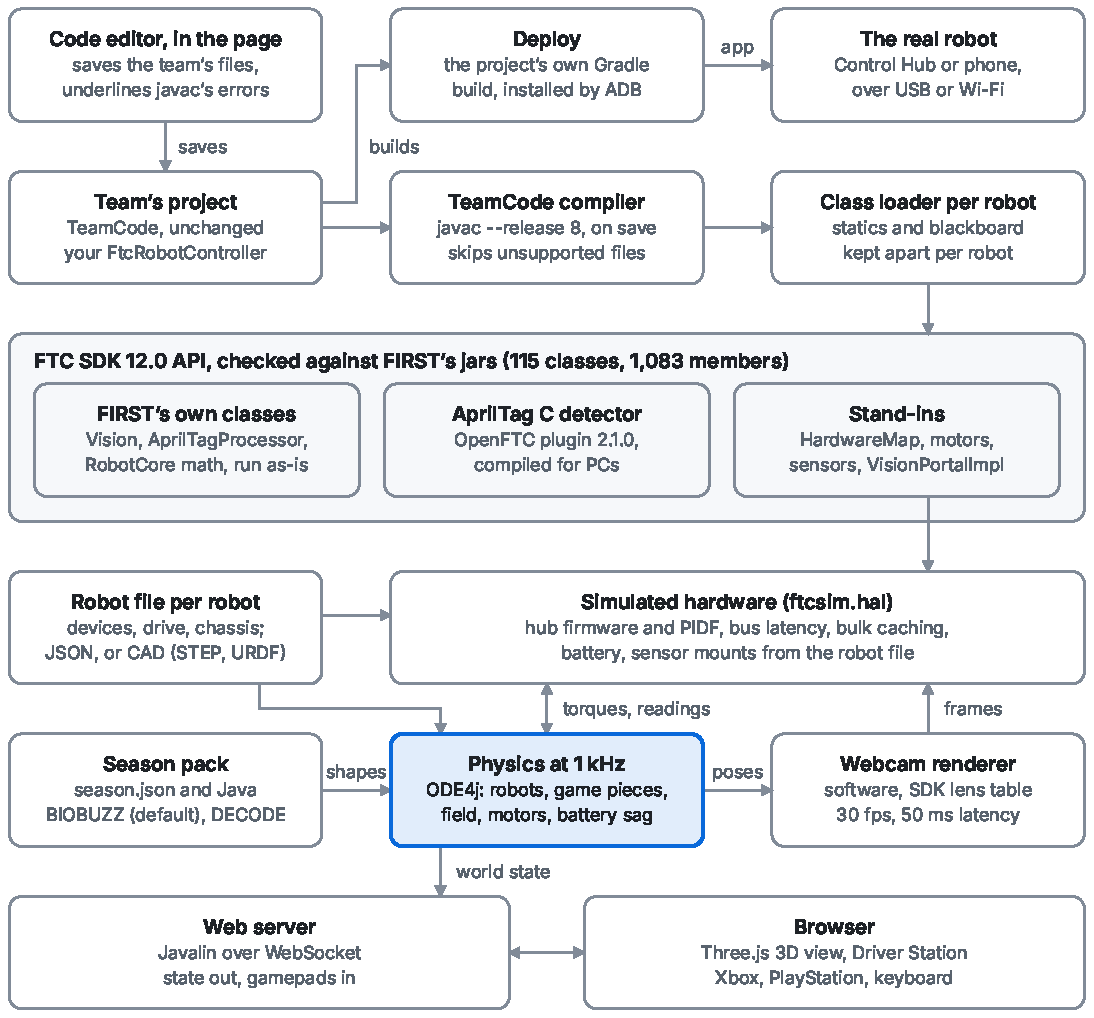
\includegraphics[width=0.967\textwidth]{figures/architecture.pdf}
\caption{\textbf{Every robot, sensor and camera reads from one 1~kHz physics world.}}\label{fig:architecture}
\end{figure*}

TeamCode is read from the team's own FtcRobotController project \citep{first2026ftcrobotcontroller}. The simulator recompiles it whenever a file is saved and loads it with a separate class loader for each robot \citep{liang1998dynamic}. TeamCode can use only the SDK 12.0 API. Behind that API, FIRST's own classes run unmodified, and stand-in classes forward hardware calls to a simulated hardware layer. That layer exchanges motor torques and sensor readings with the physics engine \citep{smith2004ode,zaschke2026ode4j} every millisecond, except that distance, color and touch sensors are read every 5~ms.

The webcam renderer draws each camera's view from the physics state, and the frames go through the VisionPortal stand-in to FIRST's vision processors. A web server streams the world state to a Three.js \citep{threejs} page, which shows the 3D view and the Driver Station and sends gamepad input back. OpModes run on their own thread, separate from physics, and STOP interrupts them. The simulator never writes to the team's project, so teams deploy to the robot with their usual tools.

The engine holds what stays the same from season to season: the field's tiles and perimeter, the physics, the robots, the SDK and the Driver Station. Everything that belongs to one game is in its season pack (\cref{sec:field}), which a command-line option selects; BIOBUZZ is the default.

\section{Field, Game Elements and Season Packs}\label{sec:field}

The simulated field follows the BIOBUZZ layout and holds its structures and 56 game pieces. The two HIVES are tuned to tip at the loads in the calibration table of FIRST's Event Field Setup Guide \citep{first2026fieldsetup}. The field and the game come from a season pack, and a second pack plays the 2025–26 game, DECODE.

\paragraph{Season packs.} A season pack is a folder holding a \code{season.\allowbreak{}json} file and, for what data cannot express, a few Java classes that are compiled with the simulator. The file describes the field as plain shapes: boxes, bars and cylinders for the structures, lines and polygons of tape, AprilTags with their centers and normals, and movers, which are parts that turn on a hinge. The physics, the webcam renderer and the browser's 3D view all build from the same shapes, so a new season needs no rendering code. A mover given a mass, center of mass, inertia and damping is a rigid body on a hinge that gravity, robots and balls move; a mover without mass moves only when the season's code turns it.

The file also lists the game pieces (diameter, mass, colors and counts, bounce, friction), the robots' starting spots and how one alliance's side maps onto the other's, how many pieces a robot may hold and its pre-load, and the human player's buttons, which the engine carries out. Where each piece starts can be data too, as in DECODE. The Java classes can add shapes computed from the data, among them shapes that stop robots but let balls through, and they run what data cannot describe: staging that follows rules, as BIOBUZZ's does, anything that has to happen at every physics step, and the counts in the Driver Station's top bar. The engine has no code for any particular game: BIOBUZZ's HIVES and their tipping, its FLOWERS and its staging rules are in the BIOBUZZ pack.

\paragraph{Field.} The layout follows the Competition Manual \citep{first2026biobuzz} and is described in the BIOBUZZ pack (\cref{fig:field-map}). The field frame has its origin at the center of the field on the tiles, with +x toward the blue alliance wall, +y away from the audience and +z up. The physics world contains the tiles, the perimeter walls, the HIVE structure (two A-frames, the axle and the sign board), the two HIVES on their pivots, and the FLOWERS against the walls. The taped areas are on the floor: LOADING ZONES as outlines and GARDENS as solid strips along the walls. Color sensors detect them, and they appear in the 3D view and in webcam images. The HIVES carry the season's tag36h11 AprilTags (IDs 30–45), which tip with the HIVE.

\begin{figure*}[t]
\centering
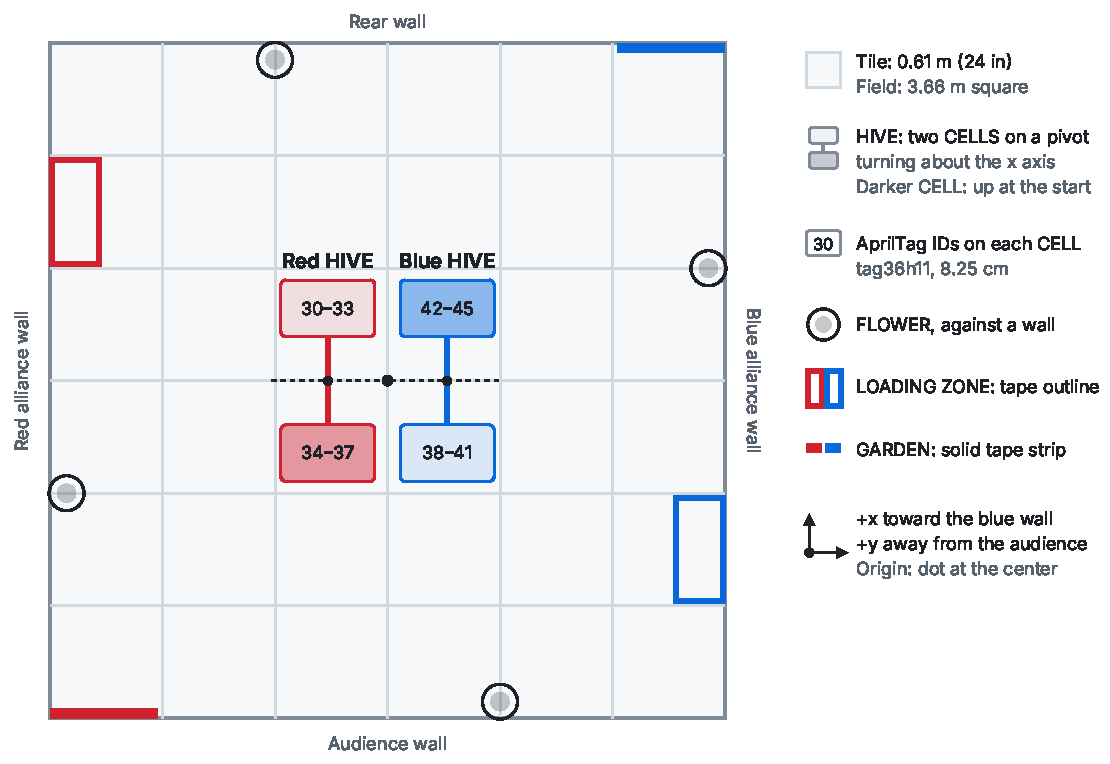
\includegraphics[width=0.981\textwidth]{figures/field-map.pdf}
\caption{\textbf{The field is the same after a half turn, with red and blue swapped.} Top view, to scale, drawn from the simulator’s field description file. Each CELL carries the IDs of its four AprilTags, and the darker CELL of each HIVE is the one that starts facing up. Turning the field half a turn about its center maps every red element onto its blue twin.}\label{fig:field-map}
\end{figure*}

\paragraph{Game pieces.} The field holds 40 POLLEN (7.1~cm) and 8 red and 8 blue NECTAR (9.1~cm), placed as in section~10.3.1 of the Competition Manual \citep{first2026biobuzz}. Loose balls roll and bounce, lose speed to air drag in flight and to rolling resistance on the tiles, and can be pushed by robots. Both kinds are perforated, like wiffle balls: the 3D view draws their holes, and the BIOBUZZ pack sets their rolling resistance to 0.12, three times the engine's default. A robot with an intake holds at most 4 balls (rule G407). A robot built from its robot file has a roller across its front that is solid to balls, so it pushes and bumps them, and while the roller spins it takes in a ball that comes within 5~cm of it; a CAD robot takes balls in at its own roller part (\cref{sec:robots}). A feeder passes them to a flywheel launcher, which throws them at about half the flywheel's surface speed and at an angle set by a hood servo.

\paragraph{FLOWERS.} Each of the four FLOWERS is an upright tube against the perimeter wall, built from boxes: a lower ring on the tiles, a middle ring above the Retrieval Opening, which faces into the field, then a funnel and a see-through tube up to the top opening, and a backstop. Balls collide with these parts. A robot's chassis stops against one box around the FLOWER that balls pass through, so only the low intake roller reaches into the Retrieval Opening. Four POLLEN start stacked single file in each FLOWER as free balls, and the weight of the stack holds the bottom one in place. A running intake takes the bottom POLLEN, and the roller of a full robot can bump it out. On the field, the POLLEN above then drop through the Retrieval Opening and roll out on their own. Simulated POLLEN are perfect spheres that would fall straight back into the lower ring, so the BIOBUZZ pack pushes each one that drops clear of the middle ring toward the front or sides at 0.5~m/s for half a second. A NECTAR dropped into a FLOWER stops on the middle ring and holds in any POLLEN put in above it.

\paragraph{HIVE model.} Each HIVE is a mover with mass: a rigid body on a pivot, limited by stops at $\pm$30° (\cref{fig:hive-seesaw}). It has two CELLS, closed at the pivot end and open at the outer end. A real HIVE stays in either position until enough weight lands in the CELL that faces up. The model gets this behavior from its mass distribution alone. The center of mass sits slightly above the pivot, so gravity holds the HIVE against whichever stop it rests on. Balls at the back of the upward CELL produce a moment in the other direction, and once it exceeds the holding moment the HIVE tips, slowed by a viscous damper.

\begin{figure*}[t]
\centering
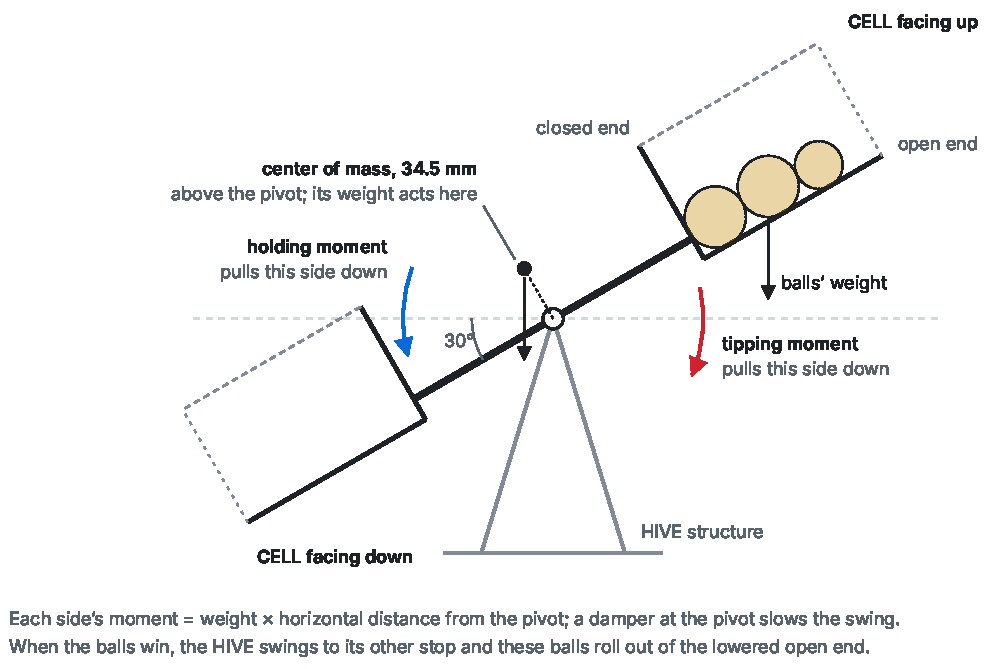
\includegraphics[width=0.874\textwidth]{figures/hive-seesaw.pdf}
\caption{\textbf{A HIVE tips when the balls’ moment beats its own holding moment.} Side view along the pivot axis, rear CELL up against its 30° stop; center-of-mass offset drawn larger than scale. The HIVE’s weight acts at its center of mass, slightly toward the lower side of the pivot, and holds it on its stop. Balls at the closed end of the upward CELL pull the other way; the curved arrows show which side each moment pulls down.}\label{fig:hive-seesaw}
\end{figure*}

\paragraph{Calibration.} The tipping point is set by one parameter, the height of the center of mass above the pivot. At 32.3~mm the model met the guide's ``Preferred'' rows, but 2 POLLEN launched by a robot onto 3 NECTAR could tip it, which the ``Necessary'' rows rule out. At 34.5~mm it meets every ``Necessary'' row (\cref{tab:hive}). We then swept the robot's distance from the CELL's open end (0.51 to 0.81~m), its launcher power and its hood angle, with the 3 starting NECTAR in the CELL. Both of 2 launched POLLEN landed in the CELL at 46 of 144 settings. At 41 of these the HIVE held, and where a 3rd POLLEN also landed, it tipped the HIVE at 30 of 31 settings. At the other 5, the first 2 POLLEN tipped it: the model meets the ``Necessary'' rows for tossed balls, but launched balls can still tip it one ball early (\code{HiveLaunchSweep}).

\begin{table}[t]
\centering
\footnotesize
\caption{The simulated HIVE against the tipping table of FIRST's Event Field Setup Guide \citep{first2026fieldsetup}.}\label{tab:hive}
\begin{tabularx}{\columnwidth}{@{}LLLL@{}}
\toprule
\textbf{Already in the upward CELL} & \textbf{Ball added} & \textbf{Guide row} & \textbf{Simulated HIVE (34.5~mm)} \\
\midrule
3 NECTAR + 1 POLLEN & 1 POLLEN, tossed & Necessary: no tip & No tip \\
6 POLLEN & 1 POLLEN, tossed & Necessary: no tip & No tip \\
3 NECTAR + 2 POLLEN & 1 POLLEN, tossed & Necessary: tips & Tips \\
7 POLLEN & 1 POLLEN, tossed & Necessary: tips & Tips \\
3 NECTAR + 2 POLLEN & 1 POLLEN, placed gently & Preferred: tips & No tip (deliberately stiffer) \\
7 POLLEN & 1 POLLEN, placed gently & Preferred: tips & No tip (deliberately stiffer) \\
\bottomrule
\end{tabularx}
\end{table}

We chose 34.5~mm because robot-launched balls are what a team sees in a match. The cost is that the model is stiffer than the guide's two gentler, hand-placed ``Preferred'' rows. Near the threshold the damper slows a tip, and the HIVE can creep off its stop for several seconds before it swings over. \code{HiveTipTest} checks every row of the table. The parameter was chosen to fit these rows, so the match holds by construction: the test guards against regressions but does not validate the model. Experiment E4 does that with loads and launches that were not used for tuning.

\paragraph{A second season: DECODE.} To check that a season can be swapped, we built a pack for DECODE, the 2025–26 game, from its Competition Manual \citep{first2025decode} and FIRST's field CAD. It uses DECODE's own field coordinates, with +x toward the audience. These are also the coordinates of the SDK's DECODE tag library, so a robot that localizes from AprilTags gets the field positions it would get on the real field. \Cref{tab:seasons} compares the two packs. An ARTIFACT that drops into a DECODE GOAL rolls down the RAMP and waits at the GATE, a mover with mass. A robot pushing the GATE's paddle toward the wall empties the RAMP, and gravity closes the GATE again. The OBELISK is a mover without mass; the pack's code turns it to a random MOTIF at every reset. The code also counts, for each GOAL, the ARTIFACTS that went through its SQUARE, those on its RAMP and how many RAMP places match the MOTIF, but it does not compute a score. The GOALS' insides, the RAMP rails (a flat plate) and the GATE lever are simplified from the CAD, and the ARTIFACT's mass (75~g, from AndyMark's listing) and bounce are estimates.

\begin{table}[t]
\centering
\footnotesize
\caption{What the two season packs contain.}\label{tab:seasons}
\begin{tabularx}{\columnwidth}{@{}>{\raggedright\arraybackslash}p{1.45cm}LL@{}}
\toprule
\textbf{Pack contents} & \textbf{BIOBUZZ (2026–27)} & \textbf{DECODE (2025–26)} \\
\midrule
Field frame & +x toward the blue alliance wall & +x toward the audience \\
Structures & HIVE structure; 4 FLOWERS that POLLEN can be taken out of; 2 HIVES (movers with mass) & 2 GOALS with RAMPS and SQUARES; 2 GATES (movers with mass); the OBELISK (mover without mass) \\
Game pieces & 40 POLLEN (7.1~cm); 8 red and 8 blue NECTAR (9.1~cm) & 36 ARTIFACTS (12.7~cm): 24 purple, 12 green \\
Each robot & Holds 4; pre-load 4 POLLEN & Holds 3; pre-load 2 purple, 1 green \\
AprilTags & 30–45, on the HIVES & 20 and 24 on the GOALS; 21–23 on the OBELISK \\
Human player & Adds one NECTAR to the LOADING ZONE & Adds one purple or green ARTIFACT to the LOADING ZONE \\
Java in the pack & 6 files (827 lines): HIVES and their tipping, FLOWERS, staging, top-bar counts & 2 files (194 lines): MOTIF, GOAL counts \\
Tests & \code{GameElementsTest}, \code{HiveTipTest}, \code{ExampleOpModesTest}, \code{SeasonsTest}, \code{MultiRobotTest}, \code{AprilTagVisionTest}; most other tests also run on this field & \code{SeasonsTest} \\
\bottomrule
\end{tabularx}
\end{table}

\section{Robots and Hardware}\label{sec:robots}

We want gains and timings tuned in simulation to carry over to the robot. Most of the modeling effort therefore goes into the drivetrain, the motors, the hub's firmware and the timing of hardware calls, and little into visual detail.

\paragraph{Robot description.} Each robot is described in a JSON file. The file sets the chassis size, mass and color, and the drive type: \code{mecanum}, six-wheel drop-center \code{tank} or four-motor \code{tank4}, with wheel diameter, wheelbase, track width, motor model and external gear ratio. It also sets the IMU's mounting and lists every device with its name, mounting position and orientation. A mechanism motor drives a load: a roller, a flywheel, an arm with gravity and hard stops, or a slide. A device can take a role (\code{intake}, \code{feeder}, \code{launcher}, \code{hood}) that connects it to game-piece handling (\cref{sec:field}). The default robot is an 18~in mecanum robot with goBILDA 312~rpm motors, 104~mm wheels, odometry pods, sensors, and a BIOBUZZ intake and launcher. A tank robot with an arm and claw is included for the classic FTC samples. A robot file can also give its own starting spot for each season, as the bundled BIOBUZZ Parking autonomous expects, and it can point at the robot's CAD model instead, as described below.

\paragraph{Rigid-body engine.} We use ODE4j 0.5.4 \citep{zaschke2026ode4j}, a pure-Java port of the Open Dynamics Engine \citep{smith2004ode}, run in-process with a fixed 1~ms step, paced to the wall clock. If the host falls more than 250 steps behind, simulated time is allowed to slip instead of running faster to catch up. On an overloaded computer the physics then lags the wall clock that OpModes measure time with, so results can depend on the computer. In published comparisons, ODE is less accurate than MuJoCo on robotics tasks \citep{erez2015simulation,collins2021review}. That is acceptable for a wheeled robot on flat tiles, and a pure-Java engine keeps the simulator in a single JVM process with no native physics library.

\paragraph{Speed.} A first run of E6 (\cref{sec:evaluation}) timed the BIOBUZZ field with all 56 game pieces on one desktop computer (AMD Ryzen 9 5900X, 12 cores, Windows 11, Java 21), each robot driving back and forth in arcs with its intake and launcher running. With robots described by hand, the physics ran at 3.0 times real time with one robot, 2.4 with two and 2.0 with four: a 1~ms step took 0.33 to 0.50~ms. Robots imported from CAD ran at 2.9, 2.3 and 1.7 times real time. One webcam frame took about 2~ms to render at 320$\times$240, 5 to 7~ms at 640$\times$480 and 23 to 29~ms at 1280$\times$720, and while a camera rendered frames back to back, the physics kept to the wall clock without skipping a step. Slower computers, laptops in particular, have not been measured.

\paragraph{Drivetrain.} The chassis is a box, and each wheel is a separate body on a hinge joint. A wheel's inertia about its axle includes the motor rotor's inertia reflected through the gearbox, which is the larger part. A mecanum wheel's rollers transmit force only along the roller axis \citep{ilon1975wheels,muir1987kinematic}. Instead of modeling individual rollers, each wheel contact sets ODE's first friction direction to the roller axis in the chassis frame and makes the perpendicular direction nearly frictionless (\cref{fig:mecanum-grip}). Gazebo users model mecanum wheels the same way \citep{gazebo2026mecanum}. A force-dependent slip term stands in for tread and roller compliance, so the wheels creep slightly under load instead of locking against each other. The six-wheel drop-center and four-motor skid-steer drives use traction wheels plus omni wheels.

\begin{figure*}[t]
\centering
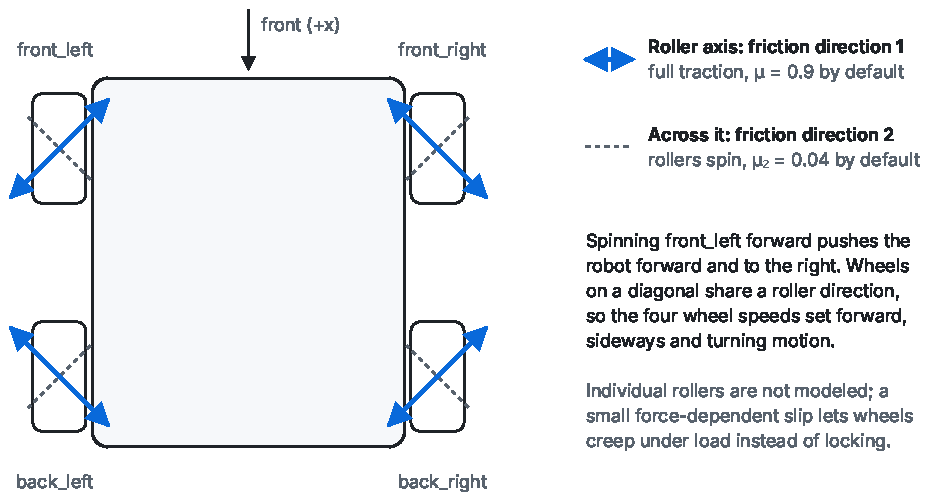
\includegraphics[width=0.820\textwidth]{figures/mecanum-grip.pdf}
\caption{\textbf{Each mecanum wheel grips only along its roller axis.} Top view of the simulated chassis, front up; directions from the robot model’s wheel setup. The solid double arrow on each wheel is the direction it grips, ODE’s first friction direction; the dashed line is the direction its rollers spin freely.}\label{fig:mecanum-grip}
\end{figure*}

\paragraph{Motors.} Each motor follows a straight-line torque–speed curve through the free speed, stall torque, and stall and free current in its vendor's datasheet. Rotor inertias are our estimates, and the REV HD Hex's geared stall torque assumes a gearbox that is 90\% efficient. Models are included for goBILDA 5203 motors at all ratios, the REV HD Hex and Core Hex, NeveRest and TETRIX. Gearbox losses are a small viscous term plus smoothed Coulomb friction. In BRAKE mode the windings are shorted; in FLOAT mode they are left open.

\paragraph{Battery.} Terminal voltage is the open-circuit voltage minus the internal resistance times the total motor current, with a 30~ms lag. Hard acceleration pulls down the voltage seen by every motor and by the robot code's own battery reading.

\paragraph{Hub firmware.} On a REV hub, the motor control loops run in the hub's firmware, not in the team's code. We implement the same modes: \code{RUN\_\allowbreak{}WITHOUT\_\allowbreak{}ENCODER}, \code{RUN\_\allowbreak{}USING\_\allowbreak{}ENCODER} with velocity PIDF, \code{RUN\_\allowbreak{}TO\_\allowbreak{}POSITION}, \code{STOP\_\allowbreak{}AND\_\allowbreak{}RESET\_\allowbreak{}ENCODER}, \code{setVelocity}, user-set PIDF coefficients and over-current reporting through \code{isOverCurrent}. As on the REV hub, the integral and derivative terms are counted in 50~ms hub control cycles, though the simulator updates them at every 1~ms step. Anti-windup \citep{astrom2008feedback} pauses integration while the output is saturated in the direction of the error and limits the integral term to half power. Encoder counts carry over from one OpMode to the next.

\paragraph{Bus timing.} On the robot, every hardware call is a message to a hub over USB or RS-485, so a control loop's period depends on how many calls it makes. The simulator adds a delay for each call, by default 1~ms per hub command and 2.5~ms per I2C read. It also implements the SDK's bulk-caching modes (\code{OFF}, \code{AUTO}, \code{MANUAL}), so code that uses bulk reads gets shorter loop times in simulation, as it does on the robot (\cref{fig:loop-timing}).

\begin{figure*}[t]
\centering
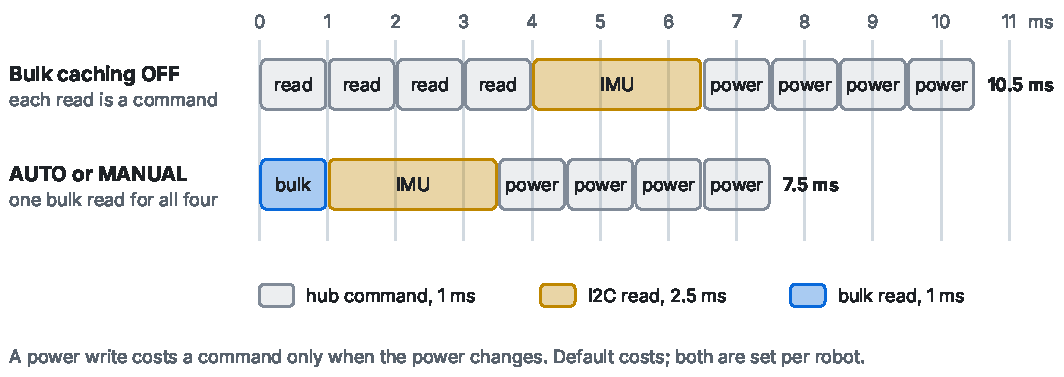
\includegraphics[width=0.941\textwidth]{figures/loop-timing.pdf}
\caption{\textbf{At the default costs, bulk reads cut this control loop from 10.5~ms to 7.5~ms.} One loop: read 4 drive encoders, read the IMU heading, set 4 changed motor powers.}\label{fig:loop-timing}
\end{figure*}

\Cref{fig:loop-timing} adds up what the simulator charges for one loop of a mecanum TeleOp at the default costs: 10.5~ms, about 95 loops per second, without bulk reads and 7.5~ms, about 133 per second, with them. Each block is one hardware call, and its width is the time charged for it. How long these calls take on a robot is for E1 and E5 to measure.

\paragraph{Sensors.} The Control Hub IMU reports yaw, pitch, roll and angular rates in the frame given by its declared mounting. The goBILDA Pinpoint computes its own odometry from the pod offsets, resolution and directions set in code. We also model the SparkFun OTOS, the REV 2~m distance sensor (by raycasting), the REV Color Sensor V3 (which reads tape and tiles), touch sensors and battery voltage. If the mounting declared in code is wrong, the readings are wrong in the same way they would be on the robot.

\paragraph{Robots from CAD.} Instead of a box chassis with load models, a robot file can point at the robot's CAD model: a STEP file \citep{iso2016step}, the format CAD programs use to export assemblies, or a URDF \citep{openrobotics2026urdf} with its meshes, which exporters for Onshape, Fusion 360 and SolidWorks write \citep{rhoban2026onshape,syuntoku2026fusion2urdf,ros2026swurdf}. The robot then looks like its CAD in the 3D view and in other robots' webcams and takes its mass properties and collision shape from the CAD. Its arms, slides, hoods and claws become rigid bodies on hinge and slider joints, driven by its motors and servos (\cref{fig:cad-import}). The devices, their mountings and the drive wheels' grip still come from the robot file, so TeamCode finds the same hardware.

\begin{figure*}[t]
\centering
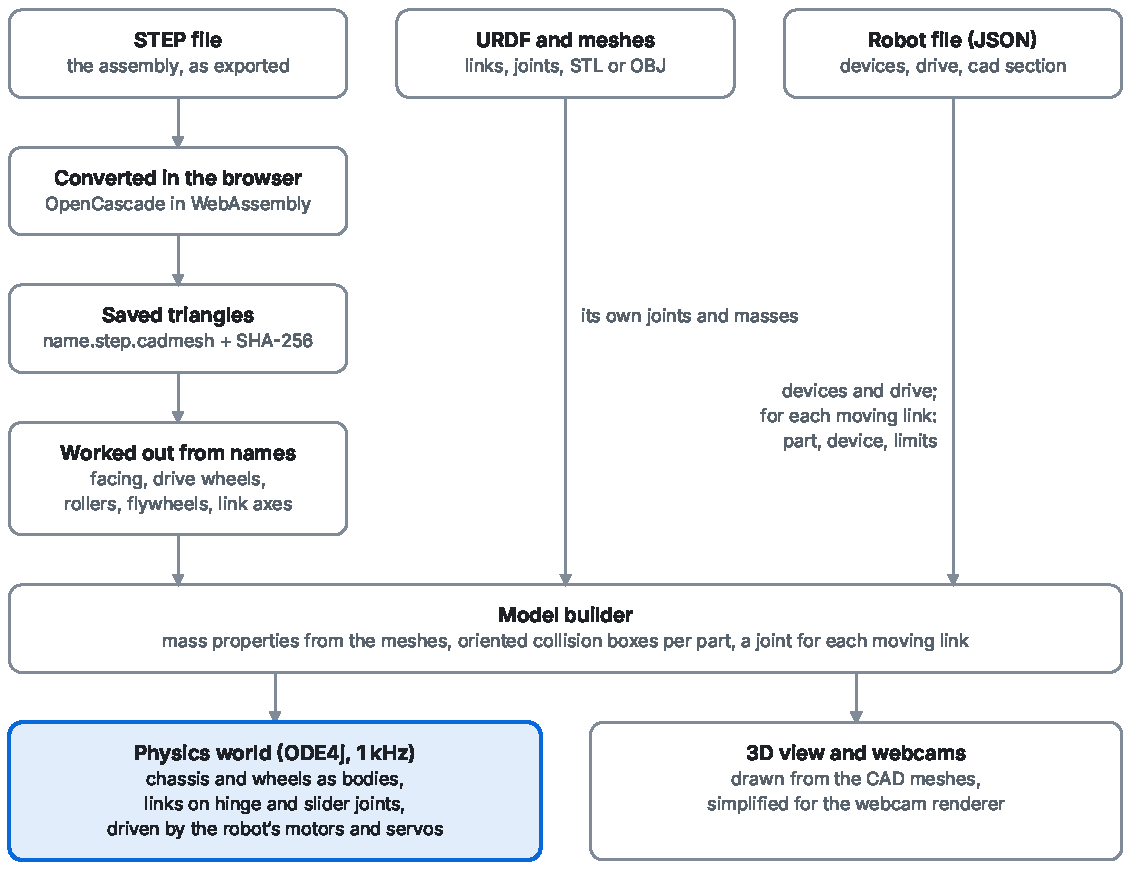
\includegraphics[width=1.000\textwidth]{figures/cad-import.pdf}
\caption{\textbf{The CAD gives the shape and mass, the robot file the devices and limits.} A STEP file goes down the left column: the browser converts it once, and the simulator works out the rest from the saved triangles and the part names. A URDF skips those steps because it already has joints and masses. Either way, the robot file adds the devices and, for each moving link, the part, its device and its limits.}\label{fig:cad-import}
\end{figure*}

\paragraph{Reading a STEP file.} OpenCascade compiled to WebAssembly (occt-import-js 0.0.23 \citep{kovacs2026occt}) converts the STEP file to triangles in the browser. The triangles are saved next to the STEP file with its SHA-256 hash, so a file is converted again only when it changes. From the triangles and the part names, the simulator works out which way is up and which is the front (up from the drive wheels, which are level and below the robot; the front from the intake or from parts named \emph{front}), which parts are drive wheels (parts named like \emph{wheel}, \emph{mecanum} or \emph{omni} that touch the floor), and which rollers and flywheels each motor turns (round parts named like the device). A STEP file does not say how a part moves, so each arm, slide or hood needs one entry in the robot file: its part name, its device, whether it slides, and its limits if it has any. A turning link's axis is taken from a round part named like a shaft, axle, pivot or hinge that is in it or touches it; a slide moves along its longest dimension unless the entry names the part to slide along. A team can also drop a STEP file on the Driver Station page, which writes a robot file with the devices and drive of the robot in use.

\paragraph{Bodies, joints and collisions.} Each part's volume, center of mass and inertia are computed from its triangle mesh by summing signed tetrahedra. For a STEP robot, the mass given in the robot file is spread over the parts by volume unless a link has its own mass; a URDF's masses can be scaled to the robot's total mass. A part collides through an oriented box along its principal axes, split into as many as eight smaller boxes when that fits a bent or curved part more closely, in the manner of OBBTree \citep{gottschalk1996obbtree}. Parts under 2~cm across, such as screws and nuts, get no box. A motor drives its joint through its torque curve and gearbox, and its encoder counts the joint's motion. A positional servo pulls its joint toward the horn angle with at most its stall torque (2.5~N·m unless set), so a heavy or blocked link lags or stalls. For the webcam renderer, other robots' meshes are simplified by vertex clustering when they have many triangles \citep{rossignac1993multi}.

\paragraph{Parameters.} \Cref{tab:params} lists the model’s main parameters, where each value comes from, and the experiment in \cref{sec:evaluation} that will test it. Apart from the motor datasheet values, the lens table from FIRST's SDK, the ARTIFACT mass from AndyMark's listing and the fitted HIVE, the values are estimates that have not been measured on a robot.

\begin{table*}[t]
\centering
\small
\caption{The model's main parameters, where each value comes from, and the experiment that will test it.}\label{tab:params}
\begin{tabularx}{\textwidth}{@{}>{\raggedright\arraybackslash}p{3.0cm}L>{\raggedright\arraybackslash}p{4.4cm}>{\raggedright\arraybackslash}p{1.4cm}@{}}
\toprule
\textbf{Parameter} & \textbf{Value} & \textbf{Source} & \textbf{Tested by} \\
\midrule
Physics step & 1~ms; at most 250 steps of catch-up & Design choice & E6 \\
Hub command time & 1~ms per command & Estimate, not measured & E1, E5 \\
I2C read time & 2.5~ms per read & Estimate, not measured & E1, E5 \\
Battery & 13.2~V open-circuit, 0.06 $\Omega$, 30~ms lag, 7~V floor & Estimate & E1, E5 \\
Drive motor, default robot & goBILDA 5203 at 312 rpm free, 24.3~kg·cm stall torque, 9.2~A stall, 0.25~A free & Vendor datasheet & E1 \\
Mecanum friction & $\mu$ 0.9 along the roller axis, 0.04 across; slip 0.002 & Estimate & E1, E5 \\
HIVE & 2.5~kg; center of mass 34.5~mm above the pivot; damping 0.35~N·m·s/rad & Mass and damping estimated; center of mass fitted (\cref{sec:field}) & E4 \\
Balls & Drag coefficient 0.5; rolling resistance 0.04 (BIOBUZZ: 0.12); launched at 0.5 of the flywheel’s surface speed & Estimate & E4 \\
Intake roller (robot file) & 3~cm radius, 4~cm ahead of the chassis; takes in a ball within 5~cm of its surface & Estimate & E4 \\
FLOWER roll-out & 0.5~m/s for 0.5~s, within 100° of the Retrieval Opening's direction & Estimate & E4 \\
Webcam & 30 frames/s, 50~ms latency; lens from the SDK calibration table & Defaults; lens from FIRST & E3 \\
CAD links & Mass spread by volume unless set; servo stall torque 2.5~N·m; slide spool 38~mm & Defaults, set per link & E5 \\
ARTIFACT (DECODE) & 75~g; bounce 0.3 & Estimate; mass from AndyMark's listing (0.165~lb) & — \\
\bottomrule
\end{tabularx}
\end{table*}

\section{Simulated Vision}\label{sec:vision}

The simulator renders camera images and runs FIRST's unmodified vision pipeline on them; it does not compute detections from geometry (\cref{fig:vision-pipeline}). In our tests, the tag poses that FIRST's \code{AprilTagProcessor} solves from simulated frames agree with the true camera-to-tag positions to within 2~mm on every axis, and with the tags' orientations to within 1.7°, for four tag poses 0.70–0.76~m from a Logitech C920 lens model. The test prints every error and fails beyond 5~mm per axis or 3° of orientation. A team's VisionPortal code, processor settings and pose calculations run through the same code as on the robot.

\begin{figure*}[t]
\centering
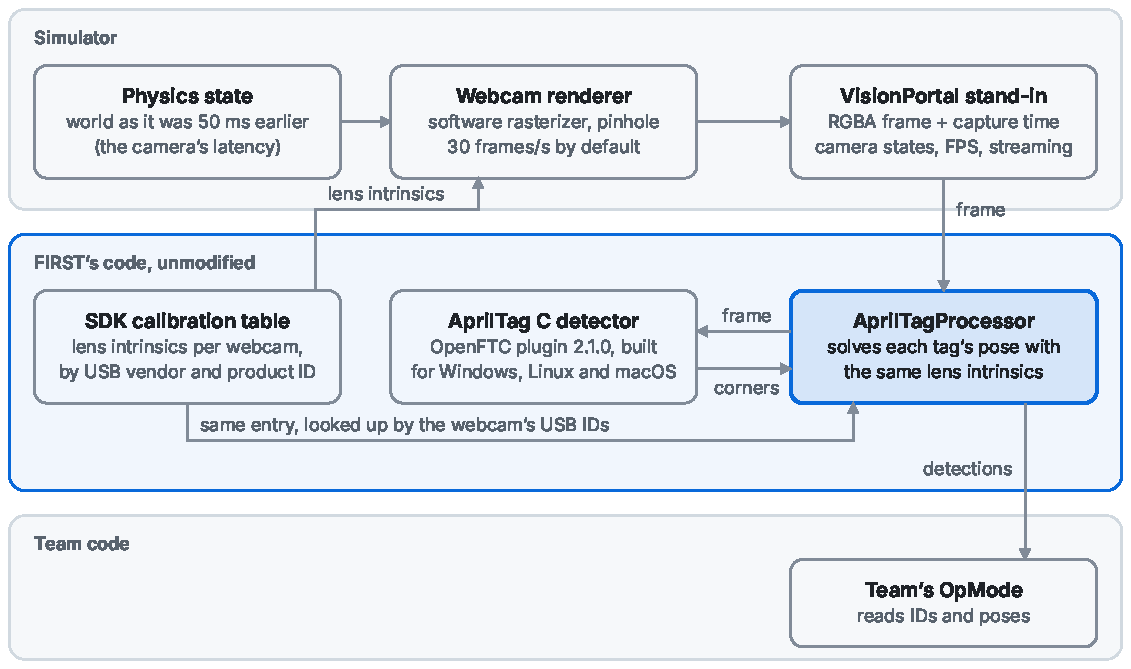
\includegraphics[width=1.000\textwidth]{figures/vision-pipeline.pdf}
\caption{\textbf{Only the image is simulated: FIRST’s code finds the tags and solves their pose.} One webcam frame, from the physics state to the detections a team’s OpMode reads. Only the top band is the simulator’s code; the middle band is FIRST’s, run unmodified. The renderer and FIRST’s AprilTagProcessor take the lens from the same calibration-table entry, so the image and the pose solver agree on it.}\label{fig:vision-pipeline}
\end{figure*}

\paragraph{Rendering.} A small software rasterizer written in Java draws each webcam's view. It draws z-buffered triangles with flat, textured or procedural floor shading, blends transparent surfaces back to front, draws balls as spheres, and interpolates texture coordinates with perspective correction. The image is split into bands of rows that are rendered on separate threads. The camera is an ideal pinhole with OpenCV's axis and pixel-center conventions \citep{hartley2004multiple,bradski2000opencv}, which is the model FIRST's pose solver assumes. The scene is built from the season pack's shapes, as the physics is; on the BIOBUZZ field it includes the HIVES with their tag36h11 AprilTags (IDs 30–45). It also contains the robots, drawn from their CAD meshes where they have them, and the balls.

\paragraph{Lens model.} Each simulated webcam takes its intrinsics from the SDK's built-in calibration table, for example the entry for the Logitech C920. FIRST's AprilTag processor finds the same entry from the webcam's USB vendor and product IDs. The renderer and the pose solver therefore use the same lens parameters, as on a robot with a calibrated webcam.

\paragraph{Timing.} Frames arrive at the camera's frame rate, 30 frames/s by default. Each frame shows the world as it was \code{latency\_\allowbreak{}ms} earlier (50~ms by default) and is stamped with that capture time, so code that compensates for camera latency can be tested.

\paragraph{Detection.} Frames pass through FIRST's Vision classes to the AprilTag C library that FIRST ships \citep{olson2011apriltag,wang2016apriltag,krogius2019flexible}, which we built from the same source for Windows and Linux on x86-64 \citep{openftc2026apriltag}. OpenCV is version 4.10.0, the version the robot uses \citep{bradski2000opencv}. The season's tag library groups the BIOBUZZ tags into FIRST's named clusters such as \code{RED SCORING}, and \code{AprilTagVisionTest} checks that this cluster's reported origin is at the CELL opening. On the DECODE field, where the GOAL tags are placed from the SDK's DECODE tag library to within 1~mm, FIRST's processor locates the camera from tag 24 to within 1~cm (the test allows 3~cm). The rest of the portal (camera states, \code{getFps()}, \code{stopStreaming()}, saving frames) is our own code. Exposure, gain, focus and white-balance settings are accepted and stored but have no effect on the image.

\paragraph{Missing effects.} The rendered frames have no lens distortion \citep{zhang2000flexible}, motion blur, sensor noise or lighting variation, so the millimeter agreement is a best case; a robot's camera will do worse. Adding these effects and randomizing them \citep{tobin2017domain} is future work (\cref{sec:limitations}).

\section{Matches and the Driver Station}\label{sec:matches}

Up to four robots share one field, two per alliance. Each is a separate Robot Controller with its own TeamCode, OpMode, gamepads, telemetry and robot file (\cref{fig:match-robots}). Robots collide and push each other, and they show up in each other's distance sensors and webcams.

\paragraph{Isolation.} Each robot's TeamCode is loaded by its own class loader \citep{liang1998dynamic}, even when two robots run the same project. Static fields, \code{OpMode.\allowbreak{}blackboard}, \code{RobotLog}'s global error and the configured bus latency are kept per robot, so one robot's code cannot affect another's, and two projects can contain classes with the same name. When a file is saved, only the robots running that project are rebuilt, and each rebuild waits until that robot's OpMode has stopped.

\begin{figure*}[t]
\centering
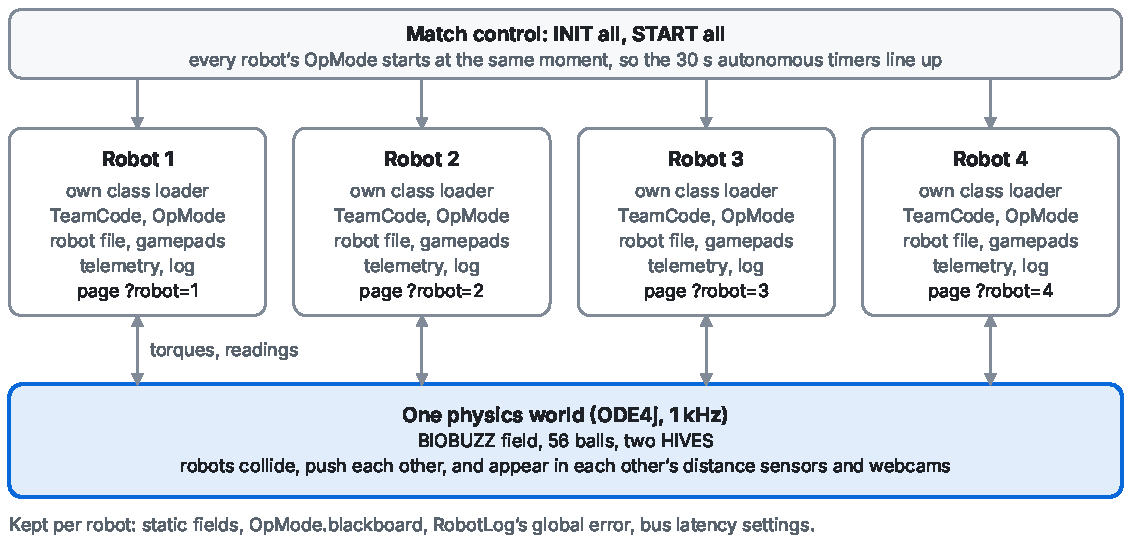
\includegraphics[width=1.000\textwidth]{figures/match-robots.pdf}
\caption{\textbf{Four robots share one physics world, but each runs its own code in isolation.} Each robot is a separate Robot Controller, and everything inside its box belongs to it alone. The robots meet only in the physics world, where they collide and sense each other, and at the match start.}\label{fig:match-robots}
\end{figure*}

\paragraph{Matches.} \emph{INIT all} and \emph{START all} act on every robot at the same moment, so their 30-second autonomous timers stay in step. Starting spots come from the season pack, two per alliance: on BIOBUZZ the blue spots are the red ones rotated 180° about the field center, and on DECODE they are the red ones mirrored. On BIOBUZZ each simulated robot starts with its 4 pre-loaded POLLEN, and the pre-loads of robots that are not simulated go in their alliance's LOADING ZONE, as the manual specifies \citep{first2026biobuzz}.

\paragraph{Driver Station.} The browser page copies the Driver Station app: OpMode lists, INIT/START/STOP with the app's rules, telemetry (with its 250~ms transmission interval and HTML format), device readouts, the robot log and a camera preview. Error messages use the app's wording, for example \emph{User code threw an uncaught exception: IllegalArgumentException - Unable to find a hardware device with name ``left\_drive'' and type DcMotor.} Xbox and PlayStation controllers connect through the browser's Gamepad API, with rumble in Chrome and Edge, and the keyboard works as a fallback. Opening the page with \code{?robot=N} shows and controls only that robot, so each driver can have a separate screen. Each robot's readout shows how many game pieces it holds against the season's limit. With several robots, each robot's card shows its TeamCode folder and battery voltage and has its own robot-file menu and STEP import; a changed robot file takes effect only while that robot's OpMode is stopped. The season sets the human player's buttons and keys and the counts in the top bar.

\section{Running Team Code}\label{sec:teamcode}

The simulated robots run the team's own TeamCode, so the simulator has to offer the same programming interface as the robot. Its SDK has no class or public member that FIRST's SDK 12.0 lacks. A test checks this for 115 stand-in classes and their 1,083 public members, so code that compiles against the simulator also compiles for the robot, unless it uses a protected member, which the test does not compare yet.

\paragraph{Three kinds of code behind the API.} \Cref{tab:layers} lists them.

\begin{table*}[t]
\centering
\small
\caption{The three kinds of code behind the SDK's API.}\label{tab:layers}
\begin{tabularx}{\textwidth}{@{}>{\raggedright\arraybackslash}p{4.2cm}>{\raggedright\arraybackslash}p{5.0cm}L@{}}
\toprule
\textbf{Layer} & \textbf{Where it comes from} & \textbf{Examples} \\
\midrule
FIRST's own classes, run unmodified & Extracted at build time from the official RobotCore 12.0.0 and Vision 12.0.0 packages on Maven Central & \code{AprilTagProcessor}, \code{ColorBlobLocatorProcessor}, navigation units and poses, matrices, camera calibration, \code{ElapsedTime}, \code{Range} \\
The AprilTag detector FIRST ships & OpenFTC EOCV-AprilTag-Plugin 2.1.0: its Java wrapper from Maven Central, unmodified, and its C source compiled for PCs \citep{openftc2026apriltag} & tag36h11 detection and pose \\
Stand-ins, same packages and signatures & Written for the simulator & \code{HardwareMap}, \code{DcMotorImpl}, \code{LynxModule}, \code{GoBildaPinpointDriver}, \code{SparkFunOTOS}, \code{VisionPortalImpl}, \code{Gamepad}, telemetry \\
\bottomrule
\end{tabularx}
\end{table*}

We replace FIRST's code only where it touches Android or hardware. For example, the build takes all of FIRST's Vision package except \code{VisionPortalImpl}, the class that opens the camera, and supplies a simulator version of that one class. Stand-ins forward calls to an internal hardware layer (\code{ftcsim.\allowbreak{}hal}) that TeamCode may not import; the compiler rejects any TeamCode file that tries.

\paragraph{API conformance.} We check the API with differential testing, which compares two implementations of one interface to find where they disagree \citep{mckeeman1998differential}. Here the two are the simulator's SDK and FIRST's published jars. \code{ApiConformanceTest} downloads the official RobotCore, Hardware and Vision 12.0.0 jars, with the EasyOpenCV jar they build on, and compares the public members of every class TeamCode can see using \code{javap}. The test fails if the simulator has a class FIRST does not ship or a public member FIRST does not declare, or if one side declares a class where the other has an interface. It leaves out \code{equals}, \code{hashCode} and \code{toString}, members whose signatures use the simulator's internal \code{ftcsim} types, which TeamCode cannot name, and the stand-ins for Android classes, which we checked by hand. It allows RobotCore's resource classes (\code{R}), which the Robot Controller app generates when it is built, and one documented exception, \code{HardwareMap}'s no-argument constructor, which team code never calls.

\code{VisionLinkageTest} checks the other direction: it resolves every class, method and field that FIRST's Vision and RobotCore bytecode refers to. A missing stand-in then shows up as a failed test instead of a \code{NoSuchMethodError} in a team's OpMode.

\paragraph{Compilation.} TeamCode is compiled in-process with the Java compiler API at the Java 8 language level, which Android Studio uses for FTC projects. A file that uses something the simulator does not model, such as EasyOpenCV cameras or Android UI, is skipped and listed with the reason, and the rest of the project still runs. All 41 official FTC sample files bundled with the simulator compile without changes or skips, and the test suite runs several of them end to end (\cref{sec:verification}).

\section{Verification}\label{sec:verification}

The simulator has 15 JUnit test classes with 91 tests, and they run on Windows, Ubuntu and macOS for every push to the main branch and every pull request. \Cref{tab:tests} lists what each one checks and what it takes to pass. Two more classes hold the measurements in this report, the HIVE launch sweep (\cref{sec:field}) and E6 (\cref{sec:robots}); \code{gradlew :engine:experiment} runs them on demand, since they take minutes and their timings depend on the computer.

\begin{table*}[t]
\centering
\small
\caption{The test classes, what each checks, and what it takes to pass.}\label{tab:tests}
\begin{tabularx}{\textwidth}{@{}>{\raggedright\arraybackslash}p{4.0cm}>{\raggedright\arraybackslash}p{5.2cm}L@{}}
\toprule
\textbf{Test class} & \textbf{What it checks} & \textbf{Pass criterion} \\
\midrule
\code{ApiConformanceTest} & Simulator SDK is a subset of the official SDK 12.0 jars & No extra class or public member (115 classes, 1,083 public members) \\
\code{VisionLinkageTest}, \code{AndroidMatrixTest} & FIRST's bytecode resolves against the stand-ins; the \code{android.\allowbreak{}opengl.\allowbreak{}Matrix} stand-in computes correctly & Every reference resolves; matrix results match \\
\code{DrivetrainPhysicsTest}, \code{RestDriftTest} & Speed, strafing, turning, \code{RUN\_\allowbreak{}TO\_\allowbreak{}POSITION}, wall contact, rest & Forward 1.2–1.95~m/s with under 1° of turn; strafe over 0.8~m/s; spin over 2~rad/s; RUN\_TO\_POSITION within 15 ticks; under 2~mm drift in 60 s at rest \\
\code{GameElementsTest} & Staging per manual 10.3.1, pushing, intake limit, launching, CELL containment; FLOWERS: the stack stays, the intake empties a FLOWER from the bottom, a full robot's roller bumps the bottom POLLEN out, a NECTAR stops on the middle ring & Counts exact; balls stay in or bounce off CELLS as specified; the intake takes all 4 POLLEN out of a FLOWER, and once the bottom one is gone at least 2 of the 3 above roll out \\
\code{HiveTipTest} & Calibration table (\cref{sec:field}), tip dumps the CELL & Every row as in \cref{sec:field} (fitted, so a regression check) \\
\code{MultiRobotTest} & Class-loader isolation, spots, pre-loads, pushing, synchronized START & Per-robot state independent \\
\code{SeasonsTest} & Every season pack loads and plays; on DECODE: staging, GOAL tags against FIRST's tag library, RAMP and GATE, human player, MOTIF, AprilTag localization & Robot stays within 3~cm of its start spot and balls stay on the field; counts exact; tags within 1~mm of the library; camera within 3~cm (observed: within 1~cm) \\
\code{CadImportTest} & STEP and URDF examples read into links, joints, wheels and masses; detection from part names; when a STEP file is converted again; CAD robots drive, lift, aim, take in and launch & Detected model matches the spelled-out one within 2~mm; forward 1.2–1.95~m/s with under 1.5° of turn; hood within 1° of its servo; ball leaves within 2~cm of the flywheel rim \\
\code{AprilTagVisionTest}, \code{CameraStreamTest}, \code{VisionPortalBehaviorTest} & Tag poses from rendered frames, live view, portal lifecycle & Each tag position within 5~mm per axis and orientation within 3° (observed: within 2~mm and 1.7°); cluster origin within 10~mm \\
\code{SampleOpModesTest} & Official samples compile and run & All 41 compile; \code{RobotAutoDriveByGyro\_\allowbreak{}Linear} ends within 0.15~m and 3° of its start \\
\code{ExampleOpModesTest} & Bundled BIOBUZZ examples: TeleOp, Pinpoint and Parking autonomous & Pinpoint auto returns within 1.5~in (38~mm) and 3° of its start (observed: 0.56~in); Parking ends within 5~cm and 3° of its target, back half in the red LOADING ZONE (observed in two runs: 4 and 10~mm, under 0.5°); from the near end, middle and far end of the shooting range, the first 2 shots land in the CELL and the 3rd tips the HIVE \\
\bottomrule
\end{tabularx}
\end{table*}

\paragraph{Continuous integration.} One GitHub Actions workflow per operating system runs the suite on JDK 21, plus JDK 17 on Ubuntu. Each run also starts the simulator through its launch script against a robot project whose path contains spaces. It then checks that TeamCode compiles with no files skipped and that the Driver Station page loads.

\paragraph{Gaps.} The AprilTag native library is built only for Windows and Linux on x86-64, so the vision tests are skipped on macOS and ARM machines. All of these tests compare the simulator with itself or with FIRST's documents, not with a physical robot. \cref{sec:evaluation} plans that comparison.

\section{Evaluation Plan}\label{sec:evaluation}

The main question is how closely the simulation matches a real robot on a real field, in its motion, control loops, sensors and game elements. Apart from a first run of E6 on one computer (\cref{sec:robots}), none of these experiments has been run yet. We set out the methods and metrics here (\cref{tab:eval}), before collecting any results.

\begin{table*}[t]
\centering
\small
\caption{Planned experiments. Only E6 has had a first run, on one computer.}\label{tab:eval}
\begin{tabularx}{\textwidth}{@{}>{\raggedright\arraybackslash}p{0.6cm}>{\raggedright\arraybackslash}p{3.3cm}L>{\raggedright\arraybackslash}p{4.0cm}>{\raggedright\arraybackslash}p{1.2cm}@{}}
\toprule
\textbf{\#} & \textbf{Question} & \textbf{Method} & \textbf{Metrics} & \textbf{Needs} \\
\midrule
E1 & How close is the drivetrain to a real one? & Run the same scripted OpModes on the robot and in simulation: straight drive, strafe, spin, \code{RUN\_\allowbreak{}TO\_\allowbreak{}POSITION} steps & Velocity and position RMSE over time; settling time; final pose error & Robot \\
E2 & Does tuning done in simulation hold on the robot? & Tune heading PID and a velocity PIDF in simulation only, deploy unchanged, repeat E1's runs & Tracking error on the robot versus in simulation; retuning needed & Robot \\
E3 & Do sensors read as on the robot? & Log IMU heading, Pinpoint odometry, distance and color readings, and AprilTag poses at measured positions, on both & Error against ground truth, robot versus simulation & Robot \\
E4 & Do game elements behave as on the field? & Launch POLLEN across the shooting range at set speeds and hood angles; load a HIVE ball by ball; take POLLEN out of a FLOWER with the intake & Landing-point error; balls needed to tip the HIVE; POLLEN that roll out of a FLOWER on their own, simulation versus field & Robot, HIVE \\
E5 & Which modeling choices matter? & Turn off one model at a time: bus latency, bulk caching, anisotropic wheel friction, battery sag; swap the hand-written robot description for the CAD import & Change in loop period and in E1–E2 metrics & E1 data \\
E6 & Does it run in real time? & Time the physics step and webcam rendering with 1–4 robots, described by hand and from CAD, and all of a season's game pieces & Real-time factor; render ms per frame by resolution & — \\
E7 & How much real team code runs in it? & Compile a sample of public FtcRobotController team repositories built against SDK 12.0 & Share of files compiled and of OpModes that start without error; skip reasons ranked & — \\
E8 & Does it help students? & Two groups write the same autonomous, one using the simulator first & Time to a working autonomous on the robot; bugs found at the field & Robot \\
\bottomrule
\end{tabularx}
\end{table*}

E1 and E2 are the main experiments. E2 answers the question teams care about most: do gains tuned in simulation work on the robot without retuning? E1 helps explain E2's outcome, and E5 shows which parts of the model are worth their cost.

E3 and E4 extend the comparison to sensors and game elements, which decide whether autonomous routines and scoring shots behave the same on the field. E4 needs a HIVE built to FIRST's field drawings.

E7 measures compatibility with real team code, not fidelity. Repositories would be sampled by a stated rule and reported in aggregate, without naming teams. E8 involves human participants and needs approval from an institutional review board before any data is collected.

\section{Limitations and Future Work}\label{sec:limitations}

The main limitation is that the simulator has not yet been compared with a physical robot; experiments E1–E4 in \cref{sec:evaluation} are meant to do that. The others are modeling assumptions and features not yet modeled.

\paragraph{Modeling assumptions.} Motors follow a straight torque–speed line, and the battery is a single internal resistance with a lag (tested by E1 and E5). Mecanum rollers are replaced by one friction direction per contact, and ODE approximates the friction at each contact (E1, E5). Hub command and I2C read times are fixed per robot instead of varying with bus load (E5). Webcams are ideal pinholes with no noise (E3). A STEP robot's mass is spread over its parts by volume unless the robot file gives link masses, and its parts collide as fitted boxes (E5). The HIVE is fitted with one parameter, and 2 launched POLLEN still tip it at 5 of the 46 settings that land them (E4). POLLEN roll out of a FLOWER because the BIOBUZZ pack pushes them, not through contact alone (E4). When the computer cannot keep up, the physics lags the wall clock that OpModes use, so heavy scenes can behave differently on slower machines (E6).

\paragraph{Not modeled.} MATCH scoring, in either season; LEDs and sounds; Limelight and OctoQuad; legacy BNO055 and Modern Robotics sensors; switchable webcams; cameras opened directly through EasyOpenCV; lens distortion, motion blur and noise in webcam images; materials and mates in CAD models. OpModes that use an unmodeled device are skipped at build time with the reason, so the rest of a project still runs.

\paragraph{Platforms.} The physics, compiler and Driver Station are pure Java or browser code, and STEP files are converted in the browser by WebAssembly. The AprilTag native library is built only for Windows and Linux on x86-64, so AprilTag detection does not work on macOS or ARM yet. OpenCV's own libraries do exist for macOS and for Linux on ARM, but vision has not been tested there.

\paragraph{Future work.}\mbox{}

\begin{enumerate}
\item \textbf{Camera realism.} Add lens distortion from each webcam's calibration coefficients \citep{zhang2000flexible}, motion blur from the robot's speed during exposure, and sensor noise. Randomizing these on each run \citep{tobin2017domain} would test vision code against the kind of variation a real camera produces.
\item \textbf{Headless batch runs.} Run OpModes faster than real time without the browser, for regression tests of team code and for automated tuning of gains.
\item \textbf{Scoring.} Score a MATCH from each season's game state (the HIVES in BIOBUZZ; the RAMPS and the MOTIF in DECODE) so autonomous routines can be compared by points.
\end{enumerate}

\section{Conclusion}\label{sec:conclusion}

We have described a simulator for the 2026–27 FTC game, BIOBUZZ. Up to four robots, each running its team's own code, play on a physics model of the field with HIVES calibrated to FIRST's setup guide. Robots can be imported from their CAD models, and the game lives in a season pack, so the previous season's game, DECODE, runs on the same engine. The models of motors, hub firmware, hardware-call timing, sensors and webcams are meant to let teams tune control code before they have a working robot. Our tests check these models against FIRST's documents and against the simulator's own invariants. Every one of the SDK's 115 classes and 1,083 public members exists in FIRST's, all 41 of FIRST's sample files bundled with the simulator compile unmodified, the HIVE meets every “Necessary” row of FIRST's table, and simulated AprilTag positions are within 2~mm of ground truth. How well they match a physical robot is still unknown, and \cref{sec:evaluation} describes how we plan to measure it.

\section*{Availability}

The source code is at \href{https://github.com/leelening/ftc-sim}{github.com/leelening/ftc-sim} under the MIT license. It needs JDK 17 or newer; continuous integration runs JDK 21 on Windows, Ubuntu and macOS and JDK 17 on Ubuntu. AprilTag detection needs Windows or Linux on x86-64. \code{gradlew test} runs the test suite of \cref{sec:verification}, and \code{-{}-{}season decode} starts the simulator on the DECODE field. This draft describes the main branch as of commit 362a7a0 (2026-11-19); no release has been tagged yet.

\bibliographystyle{unsrtnat}
\bibliography{ftcsim-references}

\end{document}
